\newpage
\section{Results}
% General structure.
% Display spectrums, try to calculate quality factor at least.
% Display some prelimary purities.
% Some stuff I probably should have calculated:
% Powers in the waveguide, peak power
\subsection{Glassgow}
This chip was used to do an initial proof of concept that the JSI of a ring resonator could be measured at high resolution. Here the aim was to explore different ring geometries and develop an intuition on how to do the experiment. The Pritel pulsed laser was used with a pulse duration of \SI{2}{\pico\second}, a FWHM of \SI{1.0}{\nano\meter} with wavelength range \SI{1530}{\nano\meter} to \SI{1530}{\nano\meter} and a peak power of \SI{100}{\watt}. Due to the pulsed laser sometimes destroying the spot size converter on the chip a \SI{3}{\decibel} attenuator was added to just after the laser output, this resulted in roughly about \SI{5}{\deci\bel\m} of power coming out of the lense fiber.
As each device on the chip has unique characteristics due to fabrication errors only some devices produced good data. Furthermore even if the spot size converters were of high quality, a ring which is under-coupled would not produce bright JSI data.

Here we present three data sets collected, each has high SNR of at least $20$ allowing for the maximum purity $P_{max}$ to be calculated with high precision. The relevant spectral scan is presented with the JSIs for reference, these are routine scans performed with the tunable CW laser typically at \SI{1}{\m\watt} of which roughly \SI{-14}{\deci\bel\m} gets into the chip. 

% RING C17
\begingroup
    \centering  
    \includegraphics[width=15cm]{/home/luka/Dropbox/cqp/report/thesis/res/glassgow/C17/graph.pdf}
    \captionof{figure}{{\bf JSI Ring C17} We calculate a quality factor of $Q \approx 25000$. In this instance the coupling loss was on average \SI{20}{\dB} and the input power of the pulsed laser was \SI{5.1}{\dB} giving a estimated power in waveguide of \SI{-5}{\dB}. The probe laser operated at \SI{1}{\m\watt}. Fitting the spectral scans of the ring resonators gives coupling parameters of the order $r=0.985$ $\tau = 0.946$ $n_{eff} = 4.136$, note these are only estimates.} 
     \vspace{3pt} \label{c17_jsi}
\endgroup

% C17 key points
% it works, SW stuff interferes and is of lower intensity, it happens before the ring


Figure \ref{c17_jsi} shows a clear response from the ring resonator at the resonant frequencies, superimposed on this there is also straight waveguide stimulated four wave mixing observed at much lower intensities. It can be deduced that much of this straight wave guide contribution happens before the ring as it is filtered at the resonance wavelength.
The asymmetry is an experimental artefact of imperfect alignment with the pump laser and some convolution with the AWG channel. This is a contribution to the low calculated $P_{max}$ value.

% RING C21
\begingroup
    \centering  
    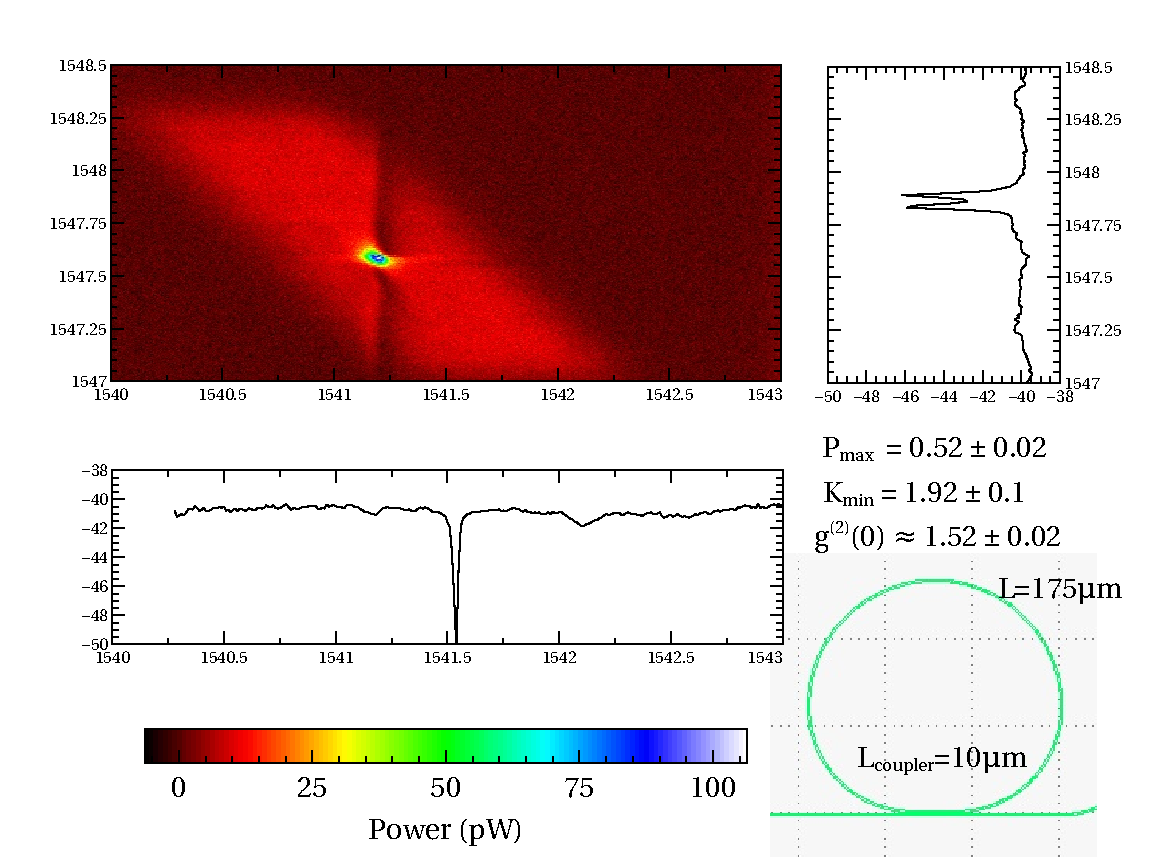
\includegraphics[width=15cm]{/home/luka/Dropbox/cqp/report/thesis/res/glassgow/C21/c21graph.pdf}
    \captionof{figure}{{\bf JSI Ring C21} We calculate a quality factor of $Q \approx 28000$. In this instance the coupling loss was on average \SI{21}{\dB} and the input power of the pulsed laser was \SI{5.5}{\deci\bel\m} giving a estimated power in waveguide of \SI{-5}{\deci\bel\m}. The probe laser operated at \SI{1}{\m\watt}. Fitting the spectral scans of the ring resonators gives coupling parameters of the order $r=0.99$ $\tau = 0.94$ $n_{eff} = 4.144$, note these are only estimates.} 
     \vspace{3pt} \label{c21_jsi}
\endgroup

% RING B32
\begingroup
    \centering  
    \includegraphics[width=15cm]{/home/luka/Dropbox/cqp/report/thesis/res/glassgow/B32/graph.pdf}
    \captionof{figure}{{\bf JSI Ring B32} We calculate a quality factor of $Q \approx $. In this instance the coupling loss was on average \SI{0}{\deci\bel\m} and the input power of the pulsed laser was \SI{0}{\deci\bel\m} giving a estimated power in waveguide of \SI{0}{\deci\bel\m}. The probe laser operated at \SI{1}{\m\watt}. Fitting the spectral scans of the ring resonators gives coupling parameters of the order $r=0.985$ $\tau = 0.946$ $n_{eff} = 4.136$, note these are only estimates.} 
     \vspace{3pt} \label{crossCompare}
\endgroup

\subsection{Toshiba}


\subsubsection{Bistability Data}
% Should be easy
\subsubsection{Pulse shaping}
% Touch on the pulse shaping experiment
\subsubsection{Power Scans}
%
\subsection{a-Si}

% Some initial joint spectrums.
% Try to calculate the quality of the rings.
% Analyse the g2(0) data